\documentclass[]{article}
\usepackage{ctex}
\usepackage{graphicx}
\usepackage{abstract}


\begin{document}
	
	\title{美赛自用攻略——论文手}
	\author{YAN}
	\maketitle
	\date{\today}
	
	\begin{abstract}
		
		美赛中摘要部分是最重要的,其次是正文。
		
	\end{abstract}
	
	\section{摘要}
		\subsection{美赛论文模板与写作方法}
			\begin{figure}[htbp]
				\centering
				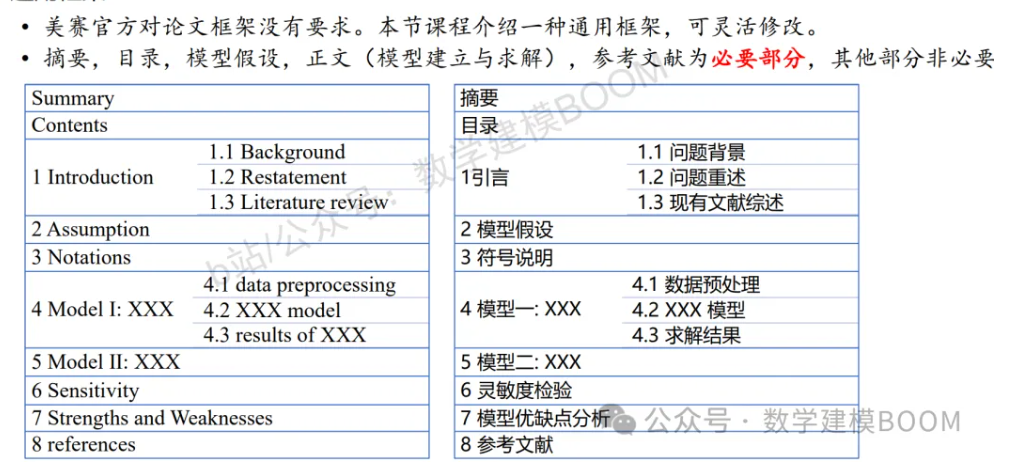
\includegraphics[width=1\textwidth]{1}
				\caption{美赛论文模板与写作方法}
				\label{fig:1}
			\end{figure}
		\subsection{比赛规则对论文的要求}
			\begin{itemize}
				\item[$\bullet$] 在第一页摘要页左上角写选择的问题,A-F之一
				\item[$\bullet$] 右上角写队伍号
				\item[$\bullet$] 论文中不得出现任何姓名和学校等信息
				\item[$\bullet$] 提交的文件为pdf格式,文件名为队伍号
				\item[$\bullet$] 文件必须小于20MB、不超过25页(包括附录等任何部分的pdf文件总页数)
			\end{itemize}
		\subsection{摘要页}
			\begin{figure}[htbp]
				\centering
				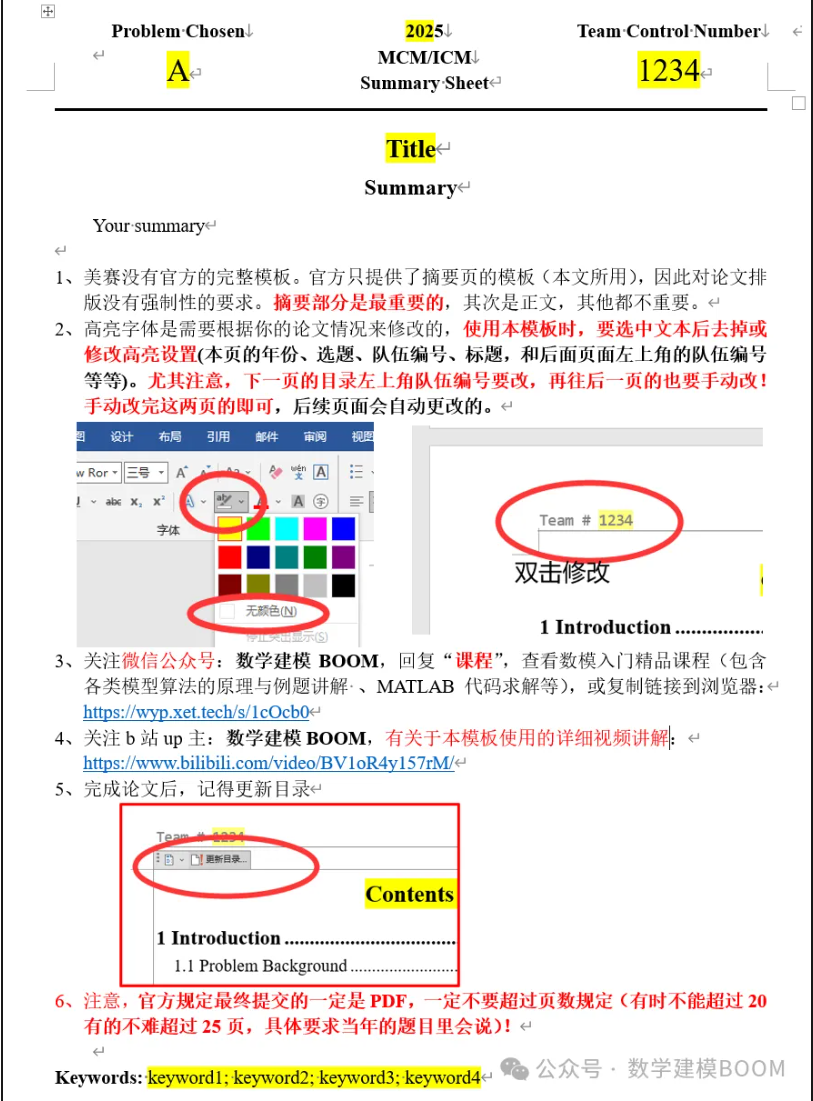
\includegraphics[width=0.8\textwidth]{2}
				\caption{摘要页}
				\label{fig:2}
			\end{figure}
	
\end{document}
